\documentclass[11pt,a4paper]{article}

% Packages
\usepackage[utf8]{inputenc}
\usepackage[T1]{fontenc}
\usepackage{graphicx}
\usepackage{hyperref}
\usepackage{color}

% Document information
\title{Rede Neurais para Espectroscopia IR}
\author{Ian Bezerra}
\date{October 2024}


\begin{document}


\maketitle


\begin{abstract}
    Usando redes Neurais para classificar funcoes organicas presentes em um espectro de IR.
\end{abstract}

\section{Introdução}
Atuais métodos de análise de espectros de IR (infravermelho) envolvem técnicas manuais e computacionais. Tradicionalmente, químicos experientes interpretam visualmente os picos e padrões do espectro, comparando-os com tabelas de referência e bibliotecas espectrais. Softwares especializados auxiliam nessa análise, oferecendo recursos de comparação automática com bancos de dados e identificação de grupos funcionais. No entanto, esses métodos podem ser demorados e sujeitos a erros humanos, especialmente para moléculas complexas ou misturas. 

Redes neurais apresentam uma quebra de paradigma na forma que reconhecemos e estudamos os padrões emergentes da natureza, pela grande maioria da história essa tarefa foi feita por mentes humanas que analisavam e modelavam tais padrões e criavam modelos e métodos determinísticos para detecção desses padrões. No entanto com o avanço de redes neurais e da computação em paralelo podemos extrair estes padrões emergentes diretamente de grandes quantidades de dados, e de certa forma “cristaliza-los” em arquiteturas de redes neurais, as quais podem ser utilizadas para generalizar estes padrões em dados não vistos previamente.

Inicialmente testamos o uso de redes neurais no reconhecimento de moléculas inorgânicas usando ondas de Raio-x(XRD) para classificação de moléculas, no entanto a simplicidade do problema, devido a natureza das moléculas inorgânicas mostrou que este problema já tinha sido mapeado de forma algorítmica, onde se pode simplesmente buscar um grande dicionário, achando o pico de maior intensidade e em seguida o segundo e assim em diante.

Com isso em mente partimos em busca de um problema mais complexo, um que requer uma certa intuição, experiência do observador. De certa forma buscamos usar a propriedade de emergência de solução desses sistemas de aprendizado de máquina para achar os padrões, dificilmente explicáveis, que criam este senso de intuição.

O problema escolhido foi a identificação de funções orgânicas, a partir de espectros de Infravermelho, adiante sera dito como isso difere do problema de classificação de moléculas.


\begin{figure}[h]
    \centering
    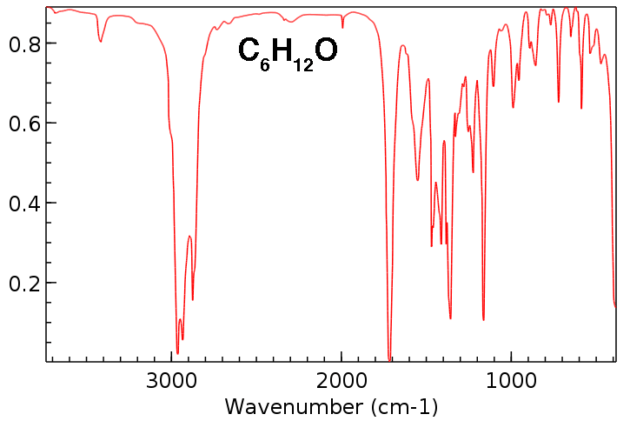
\includegraphics[width=0.8\textwidth]{Images/spec.png}
    \caption{Espectro de IR}
    \label{fig:ir_spectrum}
\end{figure}

Espectroscopia de infravermelho é uma técnica analítica versátil na química orgânica e outras ciências. Utiliza ondas eletromagnéticas infravermelhas para interagir com ligações químicas em moléculas. A absorção de energia em frequências específicas cria um espectro único, funcionando como "impressão digital" molecular. Permite identificar grupos funcionais, determinar estruturas e analisar composições. É não destrutiva, aplicável a diversos estados da matéria, sendo essencial em pesquisa e indústria.

\begin{figure}[h]
    \centering
    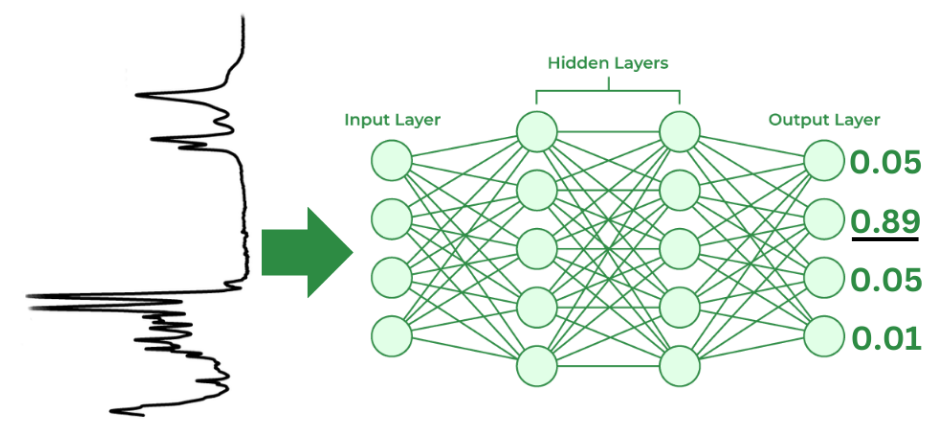
\includegraphics[width=0.8\textwidth]{Images/NN2.png}
    \caption{Rede Neural de Classificacao(Rede nao condiz com a arquitetura usada)}
    \label{fig:ir_spectrum}
\end{figure}

Em uma implementação de classificação usamos o espectro como input e usamos uma rede neural para gerar um output na ultima camada uma distribuição de probabilidade(Softmax) em cima de um dicionário de moléculas conhecidas. Assim, assumimos que a molécula com maior probabilidade é a escolha da rede neural, também é importante criar um threshold onde se à maior probabilidade for menor que este threshold, então dizemos que a rede neural “não tem certeza”. Isso pode acontecer quando colocamos como input uma molécula que não estava nos dados usados para treinar e dessa forma a rede neural não aprendeu a classificá-la.


\section{Classificacao funcoes organicas em espectros de IR}

Quando fazemos a classificação da molécula, observamos o espectro como sua impressão digital, achando similaridades entre o espectro de input e as digitais únicas das moléculas aprendidas, onde a rede neural aprende padrões únicos de cada molécula e ativa neurônios quando identifica cada padrão, subindo assim a ativação do neurônio final que representa a probabilidade da amostra ser a respectiva molécula deste índice no dicionário.

Diferentemente do problema de classificação de moléculas, a classificação de funções orgânicas dentro do espectro do IR não busca aprender a impressão digital de cada molécula, mas sim os padrões criados pela presença de uma função orgânica específica dentro de um espectro de IR. Desta forma, seria possível fornecer o input de um espectro de IR de uma molécula nunca antes vista pela rede neural, e reconhecer os padrões das funções orgânicas conhecidas presentes na molécula.

\begin{figure}[h]
    \centering
    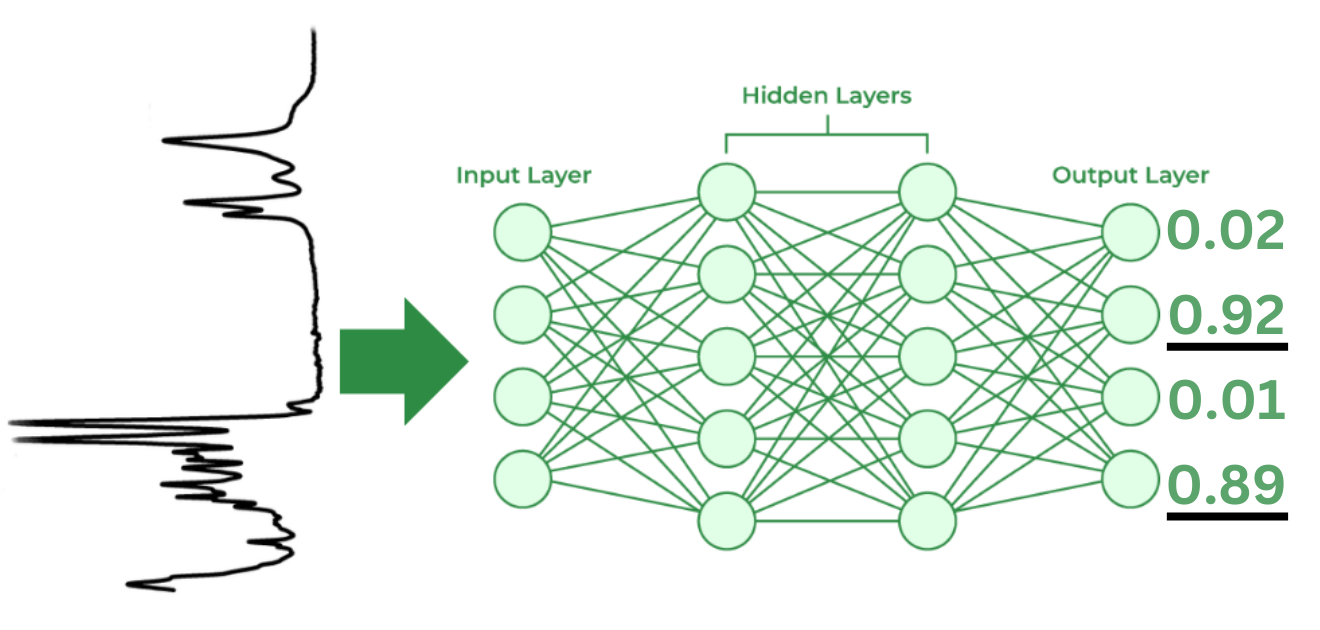
\includegraphics[width=0.8\textwidth]{Images/N2.png}
    \caption{Classificacao de funcoes organicas}
    \label{fig:ir_spectrum}
\end{figure}


No problema de classificação  de moléculas recebemos o espectro como input e criamos uma distribuição de probabilidades de ser cada molécula, que pode ser somado para 1, pois a amostra apenas pode ser uma molécula do dicionário. No entanto uma molécula pode conter mais de uma função orgânica, assim na classificação de funções orgânicas  o output final não soma para 1, mas sim cada neurônio na camada final representa uma probabilidade independente de 0 a 1 desta função orgânica estar presente na molécula. 


\section{Dados}

Na maioria dos projetos modernos de aplicações de métodos computacionais, sejam matemáticos ou de aprendizado de máquina, o uso de sistemas como crawlers/Scrappers para a aquisição de dados em grande escala. Isso majoritariamente é devido a falta de infraestrutura de APIs diretas para o download de dados em bul

\subsection{XRD cristalografia, RRUFF -  https://rruff.info/ }

Com sorte o banco de dados do RRUFF pode ser adquirido em bulk na forma de arquivos de formato “.txt” com os pontos xy, assim como o nome da molécula. Com isso foi possível construir o primeiro modelo de AI(MLP) que não vamos entrar em tanto detalhe.

\subsection{SDBS Espectrometría de IR - https://sdbs.db.aist.go.jp/ }

Este banco de dados não apresenta forma simple para o download de dados em Bulk no entanto uma implementação feita por um aluno de engenharia química da UFRJ nos possibilitou adquirir todos os dados xy assim como o nome das moléculas associadas em um banco de dados SQL, na forma “.db”.

Com isso usamos o banco de dados da PubChem para conseguir a forma simples de cada uma das moléculas, e com isso reconhecemos as funções orgânicas presentes em cada uma das moléculas. 
Futuras melhorias deste método de reconhecimento de funções orgânicas dentro dos dados serão implementadas.


\subsection{NIST Espectrometría de IR - https://sdbs.db.aist.go.jp/ }

Pela popularidade deste banco de dados, diversas implementações de crawlers já existiam, assim foi relativamente fácil conseguir o seu arquivo “.db” em SQL, no entanto o número de moléculas foi tão grande que foi necessário usar programação em paralelo em python usando a biblioteca “multiprocessing” para criar o output correspondente desejado para os dados de treinamento.


\subsection{Multiprocessing}

Usamos o processamento em paralelo para dividir o banco de dados inicial em pedaços menores, passando um pedaço para cada thread diferente, fazendo com que mais de um script de python opere de uma vez, usando assim um número predeterminado de threads do computador.

\begin{figure}[h]
    \centering
    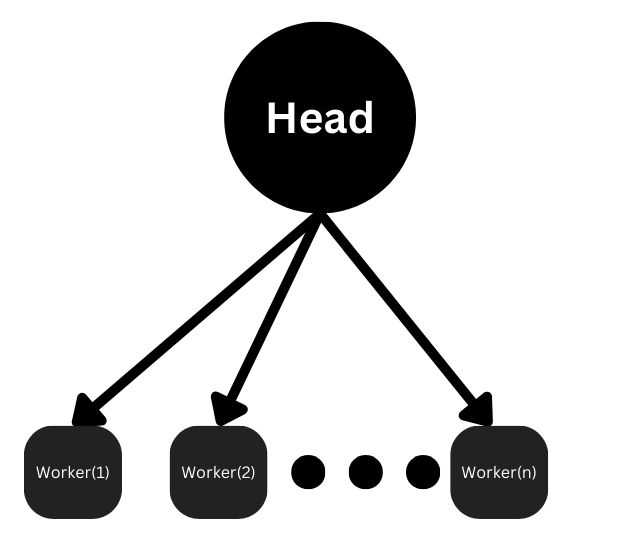
\includegraphics[width=0.5\textwidth]{Images/Multi.png}
    \caption{Multiprocessing}
    \label{fig:ir_spectrum}
\end{figure}

% No code insertion is needed here as the instructions indicate an empty code block.
\begin{verbatim}
...

data = cursor.fetchall() Importando SQL

print(f"Total number of molecules: {n_molecules}")

n = 12  # Número de workers
#n_molecules = 100

# Calcula a divisão de moléculas em n grupos
group_sizes = [n_molecules // n] * (n - 1)
group_sizes.append(n_molecules - sum(group_sizes))

print(f"Number of groups: {n}")
print("Molecule distribution:")
for i, size in enumerate(group_sizes, 1):
    print(f"n{i} = {size}")
#print(f"Número total de moléculas: {sum(group_sizes)}")
#print(group_sizes)
#print(f"Amostra de dados: {data[1]}")

irange = []
for i in range(len(group_sizes)):
    start = sum(group_sizes[:i]) + 1
    end = sum(group_sizes[:i+1])
    irange.append([start, end])

#print("irange:")
#print(irange)

# Lista de tuplas contendo nome do processo e array para passar
processes = []
i = 1
for slice in irange:
    slice.append(i)
    processes.append(('fworker2.py', slice))
    i += 1
print("Processes:")
print(processes)

# Criando um pool de processos
with Pool(processes=n) as pool:
    # Mapeia a função run_process para a lista de processos
    pool.map(run_process, processes)

#Apos concluir os processos
print("Todos os processos foram concluídos.")

\end{verbatim}

\section{Labels/Rótulos}

Para treinar redes neurais é necessário conter um conjunto de dados rotulados, com os respectivos, inputs para a rede e output “perfeito” esperado, note a nuance nesta palavra, a rede neural irá tratar os respectivos rótulos como o output perfeito a qual ele deve se assemelhar, isso gera uma dependência extremamente grande em dados que contenham não apenas um input compreensível e padronizado mas também dados extremamente bem rotulados, pois as possíveis imperfeições dos rótulos serão interpretados como perfeições a serem aprendidas pela rede neural.

\subsection{Primeira Tentativa de adquirir os rótulos}

Aqui apresentamos a estrutura do worker que cria os vetores como rótulos com índices correspondentes a o dicionário de funções orgânicas, e 1 ou 0 caso esta molécula tenha ou não a presença desta função orgânica.

\begin{verbatim}

...

def identify_functional_groups(smiles):
    mol = Chem.MolFromSmiles(smiles)
    if mol is None:
        return "Invalid SMILES string"

    functional_groups = []
    patterns = {
        "Alkyl halide": "[C][F,Cl,Br,I]",
        "Alcohol": "[OX2H]",
        "Aldehyde": "[CH1](=O)[#6]",
        "Ketone": "[#6][CX3](=O)[#6]",
        "Carboxylic acid": "[CX3](=O)[OX2H1]",
        "Ester": "[#6][CX3](=O)[OX2H0][#6]",
        "Ether": "[OD2]([#6])[#6]",
        "Amine": "[NX3;H2,H1,H0][#6]",
        "Amide": "[NX3][CX3](=[OX1])[#6]",
        "Nitro": "[N+](=O)[O-]",
        "Nitrile": "[C]#N",
        "Sulfide": "[#16X2H0]",
        "Sulfoxide": "[#16X3](=[OX1])",
        "Sulfone": "[#16X4](=[OX1])(=[OX1])",
        "Phosphate": "[P](=O)([O-])([O-])",
        "Phenol": "[OX2H][c]",
        "Imine": "[CX3]=[NX2]",
        "Alkene": "[CX2]=[CX2]",
        "Alkyne": "[CX2]#[CX2]",
        "Thiol": "[SX2H]",
        "Acyl chloride": "[CX3](=[OX1])[Cl]",
        "Anhydride": "[CX3](=[OX1])[OX2][CX3](=[OX1])",
        "Lactam": "[NX3R][CX3R](=[OX1])[#6R]",
        "Aromatic": "[a]"
    }

    for name, smarts in patterns.items():
        pattern = Chem.MolFromSmarts(smarts)
        if pattern and mol.HasSubstructMatch(pattern):
            functional_groups.append(name)

    # Additional checks for specific structures
    if mol.HasSubstructMatch(Chem.MolFromSmarts('[R]')) and not any(group in functional_groups for group in ["Aromatic", "Lactam"]):
        functional_groups.append("Alicyclic")

    return functional_groups



def generate_functional_group_vector(functional_groups):
    all_groups = [
        "Alkyl halide", "Alcohol", "Aldehyde", "Ketone", "Carboxylic acid",
        "Ester", "Ether", "Amine", "Amide", "Nitro", "Nitrile", "Sulfide", 
        "Sulfoxide", "Sulfone", "Phosphate", "Phenol", "Imine", "Alkene", 
        "Alkyne", "Thiol", "Acyl chloride", "Anhydride", "Lactam", 
        "Aromatic"
    ]
    
    vector = [1 if group in functional_groups else 0 for group in all_groups]
    return vector

...

\end{verbatim}


%----------------------------------------------


\subsection{Segunda Tentativa de adquirir os rótulos}

No entanto, ao analisar os vetores correspondentes, foi visto que os rótulos estavam com um grande índice de erro, checando mais exemplos concluímos que um jeito melhor de conseguir os rótulos a partir dos nomes ou do smiles seria necessário. Assim usamos o módulo pyCheckmol. (Veja PDF Associado)


O pyCheckmol é uma biblioteca Python que implementa funcionalidades similares ao programa Checkmol, originalmente desenvolvido em Pascal. O projeto, disponível em \url{https://github.com/jeffrichardchemistry/pyCheckmol}, visa fornecer uma alternativa em Python para a detecção de grupos funcionais em moléculas.

Principais características do pyCheckmol:

\begin{itemize}
    \item Implementa a detecção de grupos funcionais usando SMARTS patterns, similar ao Checkmol original
    \item Utiliza a biblioteca RDKit como base para manipulação de estruturas moleculares
    \item Suporta entrada de moléculas em formato SMILES
    \item Detecta diversos grupos funcionais comuns em química orgânica
    \item Fornece uma API simples e fácil de usar em Python
\end{itemize}

%----------------------------------------------

\section{Implementação}

\subsection{Arquitetura da Rede Neural}

{\color{red}(EM ANDAMENTO, APENAS NOTAS INICIAIS...)}\\
{\color{red}(VER ARQUIVO IR\_NN(v0.1).ipynb)(MLP)}

Futuramente, pretendemos explorar o uso de Redes Neurais Convolucionais (CNN) para melhorar o desempenho do modelo. As CNNs são especialmente eficazes no processamento de dados com padrões espaciais ou sequenciais, e podem ser mais adequadas para análise espectral do que as redes neurais tradicionais (MLP). 


A arquitetura inicial da rede neural implementada é definida pela seguinte classe em PyTorch:

\begin{verbatim}

class ImprovedNN(nn.Module):
    def __init__(self):
        super(ImprovedNN, self).__init__()
        self.fc1 = nn.Linear(980, 512)
        self.fc2 = nn.Linear(512, 256) 
        self.fc3 = nn.Linear(256, 64)
        self.fc4 = nn.Linear(64, 24)
        
        self.ln1 = nn.LayerNorm(512)
        self.ln2 = nn.LayerNorm(256)
        self.ln3 = nn.LayerNorm(64)
        
        # He initialization
        nn.init.kaiming_normal_(self.fc1.weight, nonlinearity='leaky_relu')
        nn.init.kaiming_normal_(self.fc2.weight, nonlinearity='leaky_relu')
        nn.init.kaiming_normal_(self.fc3.weight, nonlinearity='leaky_relu')
        nn.init.kaiming_normal_(self.fc4.weight, nonlinearity='leaky_relu')

    def forward(self, x):
        x1 = F.leaky_relu(self.ln1(self.fc1(x)))
        x2 = F.leaky_relu(self.ln2(self.fc2(x1))) + x1  # Residual connection
        x3 = F.leaky_relu(self.ln3(self.fc3(x2)))
        out = self.fc4(x3)
        return out
\end{verbatim}




\section{Conclusão}

...

%------------------------------------------------------------------------
% Comment out the bibliography-related commands if you don't have a .bib file
% \bibliographystyle{plain}
% \bibliography{references}

\end{document}
